%=========================================================================
% (c) Michal Bidlo, Bohuslav Křena, 2008
%emitter priklad

\definecolor{gray}{gray}{0.5}
\newcommand{\todo}[1]{\textcolor{red}{textcolor\:} \TODO{gray}{#1}}

\chapter{Introduction}
	(\textasciitilde2 ns)

	During the past two decades, there has been an increasing amount of new network architectures being proposed and researched. Why should we need them and what's the current state of the art in the field of network architecture?

		\section{Motivation}
		\section{Thesis Structure}


\chapter{Current State of The Internet}
	(\textasciitilde6 ns)
	\section{A Brief History}
	\section{Current Shortcomings and Weaknesses}

\chapter{Overview of Alternative Architectures}
	(\textasciitilde3 ns)
	\section{Design Approaches}
		 clean slate (e.g. RINA) x partial/evolutionary (e.g. DiffServ, LISP)
	\section{Research Initiatives}
		\begin{itemize}
		\item Future Internet Research and Experimentation (FIRE) -- projects in 2008, 2011
		\item Future Internet testbeds / experimentation between BRazil and Europe (FIBRE)
		\item DARPA NewArch
		\end{itemize}

		Ongoing projects: CCNx, NDN, RINA, NEBULA, MobilityFirst, XIA

\chapter{Named Data Networking}
	(\textasciitilde8 ns)
	\section{Premise}
		As described in section 2.1, the current Internet has its roots in telecommunication technology as this was the only area from which any inspiration could be taken. Because of this, technology of the Internet has been built on the paradigm of host-to-host communication. This can be visually presented on a "hourglass model", which indicates that while there's a wide array of technologies in use in the lower and higher layers, the hourglass's thin waist of end-to-end communication is the key static part binding different networks together.

		\begin{center}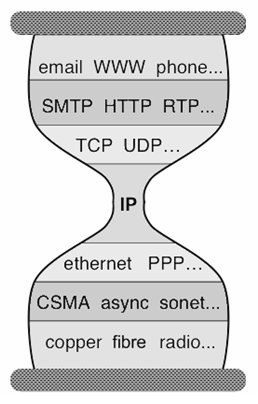
\includegraphics[width=0.2\textwidth]{media/ndn_hourglass1.jpg}\end{center}

		Building the internet as a communication network was an obvious choice, especially since most of communication of the early ARPANET consisted of connecting terminals to mainframes and executing remote procedures on them.

		However, while the basic paradigm of host-to-host communication hasn't changed, the way we use the Internet has gone in an entirely different direction: the Internet has become mostly a content distribution network. Since the mechanism of communication over the Internet is based on creating and maintaining end-to-end connections, this creates an enormous amount of data redundancy.

		Named Data Networking proposes a solution for the problem: instead of working with the source/destination node identifiers, the "thin waist" of the Internet should work with names of data chunks.

		\begin{center}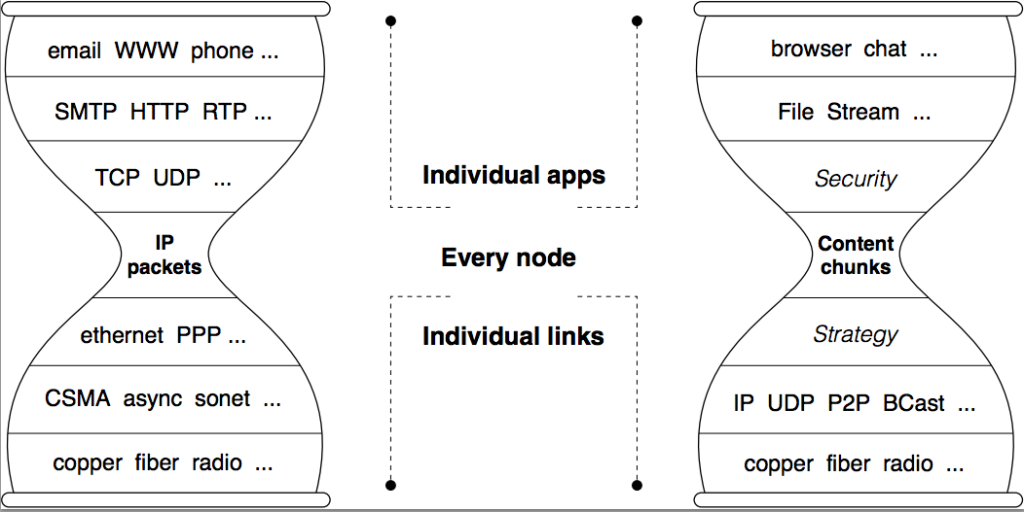
\includegraphics[width=0.6\textwidth]{media/ndn_hourglass2.png}\end{center}

	\section{Concepts}
		\subsection{The Building Blocks}
			The NDN architecture specifies:
				\begin{itemize}
				\item two types of packets: an interest packet (containing the name of desired data) and a data packet (containing the requested data)
				\begin{center}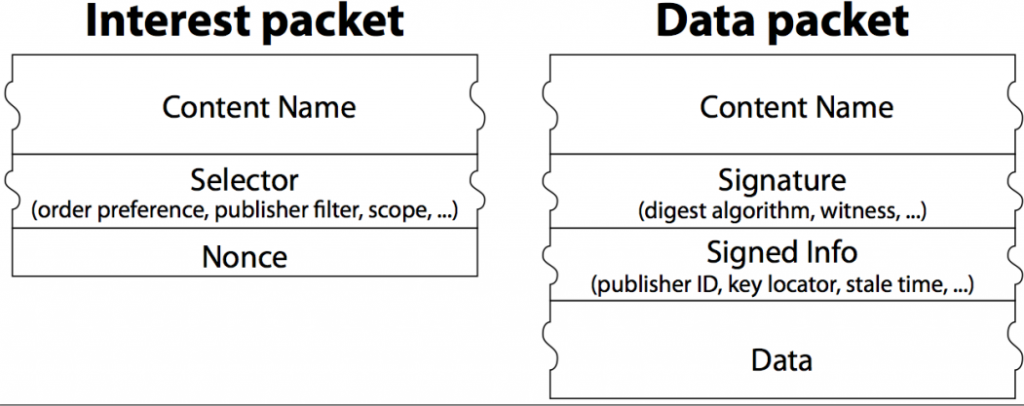
\includegraphics[width=0.6\textwidth]{media/ndn_packets1.png}\end{center}
				\item two types of hosts: a consumer (data requester) and a producer (data provider)
				\item a router maintaining three fundamental data structures:
					\begin{itemize}
					\item Forwarding Information Base (forwarding table)
					\item Pending Interest Table (maintaining currently active requests)
					\item Content Store (data cache)
					\end{itemize}
					\begin{center}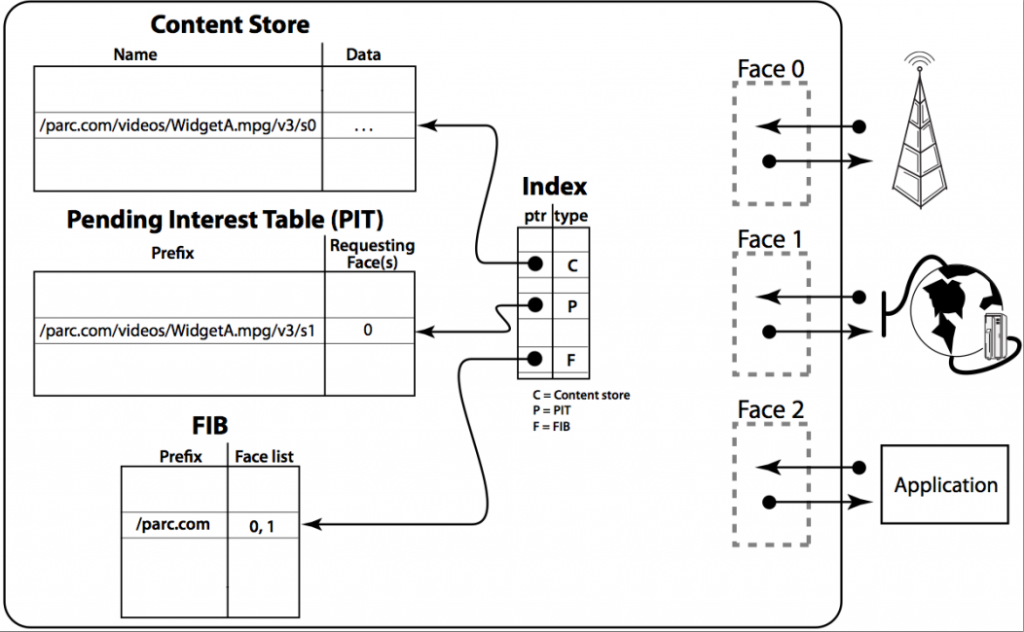
\includegraphics[width=0.6\textwidth]{media/ndn_router1.png}\end{center}

				\end{itemize}

			\subsection{The Communication Model}

			Communication in NDN is driven by the data receiver, i.e. consumer.

			\begin{enumerate}
			\item The consumer sends out an "interest packet" containing the name of the desired data.
			\item When a router receives the interest packet, it first consults its Content Store for requested data.
				\begin{itemize}
				\item If the data requested by the interest packet are present, they are returned in the direction of the requesting interface.
				\item Otherwise, it'll look up the Pending Interest Table.
					\begin{itemize}
					\item If there's an entry present for the named data request, the entry is updated by adding the originating interface into the list of requesting interfaces, thus aggregating the new request together with an existing one.
					\item Otherwise, a new entry is inserted, a FIB lookup is made and the interest packet is forwarded to interface(s) returned by the FIB.
					\end{itemize}
				\end{itemize}
			\item A data packet is returned to the router by either the producer or another router with cached data. The router finds a matching PIT entry and forwards the data to all interfaces listed in the PIT entry. The PIT entry is then removed and data are cached into the Content Store.
			\end{enumerate}

	\section{Implications}
		\subsection{Data Caching}
			The most significant feature of NDN is its native support for caching all sorts of data inside the network itself. While this should be beneficial mostly for static data such as web pages and images, dynamic content could take advantage of this as welll in case of multicasting or packet retransmission on packet loss.

		\subsection{Routing and Forwarding}
			NDN routes and forwards packets on names, which eliminates four problems caused by address forwarding in the IP architecture: address space exhaustion, NAT traversal, mobility, and address management.
			\begin{itemize}
			\item There is no address exhaustion problem since the namespace is unbounded.
			\item There is no NAT traversal problem since a host does not need to expose its address in order to offer content.
			\item Mobility, which requires changing addresses in IP, no longer breaks communication since data names remain the same.
			\item Finally, address assignment and management is no longer required in local networks, which is especially empowering for embedded sensor networks.
			\end{itemize}

			Since the forwarding mechanism otherwise bears a strong resemblance to the forwarding mechanism in IP networks, lot of the existing research on IP routing could be applied to NDN as well: protocols like BGP, IS-IS or OSPF can be, for the most part, reused with minor modifications (e.g. routers would announce name prefixes instead of IP prefixes).

		\subsection{Security}
			While TCP/IP with its end-to-end communication paradigm relies on setting up a secure channel between two hosts and transmitting data through it, NDN requires each data chunk to be signed together with its name. Thus, since security is built into the data itself, there's no need for a direct host-to-host secure channel to be created.

	\section{Current State of Implementation}

\chapter{Recursive InterNetwork Architecture}
	(\textasciitilde8 ns)
	\section{Premise}
		In 2008, computer scientist John D. Day has published a book that marked the culmination of his long-time goal of rediscovering the way we think about computer networks. The book was called Patterns in Network Architecture and in it, Day singlehandedly proposed a clean-slate approach to computer architecture that aims to get rid of most of TCP/IP's drawbacks.

		The book can be roughly divided into two separate parts: in the first part, Day attempts to decompose mechanisms used in TCP/IP to their basic parts and put them into historical and socio-economical context. He eventually discovers that the currently prevalent layered approach to network architecture is needlesly complex, because each layer consists of the same mechanisms acting on a different scope.

		The second part takes into account all of the facts discovered in the first part and uses them as foundations to build an entirely new concept of network architecture from scratch: the recursive IPC model (originally Network IPC Architecture, NIPCA).

		RINA (Recursive InterNetwork Architecture) is a currently researched network architecture based on fundamental principles described by Day.


	\section{Concepts}
	\section{Implications}
	\section{Current State of Implementation}

\chapter{Implementation of Relaying and Multiplexing Task}
	(\textasciitilde10 ns)
	\section{OMNeT++}
	\section{RINASim Library}
	\section{Relaying and Multiplexing Task}
	\section{Implementation Design}

\chapter{Testing and Evaluation}
	(\textasciitilde4 ns)

\chapter{Conclusion \& Future Development}
	(\textasciitilde1 ns)
